\listfiles
\documentclass[twoside,12pt]{article}
\newcommand{\dataset}{{\cal D}}
\newcommand{\fracpartial}[2]{\frac{\partial #1}{\partial  #2}}
\usepackage{hyperref}
\usepackage{enumerate}
\usepackage[top=2in, bottom=1.5in, left=0.85in, right=0.5in]{geometry}
\usepackage[hyphenbreaks]{breakurl}
%\usepackage[pdfstartview=FitH,pdfstartpage=13,pdfpagemode=UseNone]{hyperref}
\usepackage{amsfonts}
\usepackage{graphicx} 
\usepackage[linesnumbered,ruled]{algorithm2e}
\usepackage{float}
\usepackage{amssymb,amsmath}
\usepackage{mdwlist }
\usepackage{color}
\definecolor{darkblue}{rgb}{0.0,0.0,0.5}
\newtheorem{Dfn}{Definition}
\hypersetup{colorlinks,breaklinks,
            linkcolor=darkblue,urlcolor=darkblue,
            anchorcolor=darkblue,citecolor=darkblue}
\newcommand{\sign}{\text{sign}}
\begin{document}

\title{Learning Algorithms, Project 1}
\author{Arya Iranmehr, Mohsen Malmir, Erfan Sayyari}
\maketitle

\section{Introduction}
Logistic regression is one of the simplest linear classifiers. This model is linear, and thus inherently limited to problems that are linearly separable. Despite these limitations, We found logistic regression to be very powerful. For some problem in our research, when we used logistic regression for classification, we found it to be at least as good as SVM. For these reasons, we were very eager to dig into the details of implementing logistic regression. The result is a python class called {\it LogisticRegression}, which implements both regularized stochastic gradient descent and regularized L-BFGS for training. This class adapts the same interface used by {\it sklearn} classifiers, so it can be used in conjunction with {\it sklearn} feature extractors and other classifiers  in  pipelines. We hope to continue our work to the end of this course and implement different projects to provide an educational library of different classifiers.
\section{Design and Analysis of Algorithm}
Objective function
\begin{equation}
LCL=\sum_{i:y_i=1} \log p_i +\sum_{i:y_i=-1} \log (1-p_i)
\label{eq:LCL}
\end{equation}

Partial derivative
\begin{equation}
\nabla_j=\frac{\partial LCL }{\partial \beta_j}LCL=\sum_{i} (y_i-p_i)x_{ij}
\label{eq:pLCL}
\end{equation}

Stochastic gradient $\tilde{\nabla}$ for the stochastic mini-batch $\Omega$
\begin{equation}
\tilde{\nabla}_j=\frac{\partial LCL }{\partial \beta_j}LCL=\sum_{i \in \Omega} (y_i-p_i)x_{ij}
\label{eq:pLCL}
\end{equation}
\subsection{Stochastic Gradient Descent}
The Stochastic Gradient Descent (SGD) method approximates objective function, simply by restricting the training set to a mini-batch, i.e. random sample. 
This makes a huge difference when the training set is large and can not be fitted into memory. We implemented SGD so that the size of mini-batch could be set\footnote{When size of mini-batch is very small, e.g. 1, the stochastic gradient become noisy leading to slow rate of convergence. On the other hand, we can choose to use larger mini-batch size to reduce the variance of the gradient, which makes gradient computation more costly.} to achieve desirable rate of convergence.

\subsection{LBFGS}
We used the {\it fmin\_l\_bfgs\_b} from { \it scipy.optimize} package, which implements the limited memory {\it BFGS} algorithm and is written by Ciyou Zhu, Richard Byrd, and Jorge Nocedal. This function takes as input the function to be minimized, which is in this case the negative of regularized conditional log-likelihood,
\begin{equation}
RLCL = \sum_{i=1}^N y_i \log(P_i) + (1-y_i)\log(1 - P_i) - \mu \|\beta\|_2^2
\end{equation}
where 
\begin{equation}
P_i = \frac{1}{1+e^{-\sum_{j=1}^d \beta_j x^i_j}}
\end{equation}
Is the probability of the $i$th sample $x^i$ belonging to class with label 1. 
\section{Design of Experiments}
\subsection{SGD}
\subsubsection{Initialization}
\subsubsection{Preprocessing}
\subsubsection{Grid Search}
\subsubsection{Performance Measure}

\subsection{L-BFGS}
For testing our implementation of training with L-BFGS, we used the gender detection dataset mentioned in the homework. This is a dataset with more than 800 features and less than 600 samples, meaning that there are many features that are redundant. The data files show that the input data for training and testing are both very sparse, this increases the potential for over-fitting in the case of logistic regression. However, as we mentioned before, regularization comes to our help to prevent over-fitting.
\subsubsection{Initialization}
The initialization of the parameters is limited to the weight vector $beta$, which is the decision boundary for logistic regression. In order to select this parameter, we used grid search over different values $[0.,1e-5,1e-4,1e-3,1e-2,1e-1,1.,10]$. One might say that the effect of initial value for $\beta$ might be alleviated by choosing the $\mu$, the weight decay parameter for regularization, so there is no need for the initial value. However, since we are only searching over a small  set of values for $\mu$, introducing the initial value for $\beta$ helps to search the problem space more widely.
\subsubsection{Preprocessing}
The only preprocessing we used was the scaling, which subtracts the mean vector of the data and scales each dimension to unit variance. This helps to keep the changes in different dimensions of $\beta$ in almost the same range.
\subsubsection{Grid Search}
For grid search, We used the class {\it sklearn.grid\_search.GridSearchCV}. The benefit of using this class is that it also implements cross validation, so we can perform grid search and model selection at the same time. This class accepts a classifier as input and the number of folds for cross validation, and performs K-fold cross validation to select the best model.
\subsubsection{Performance Measure}
For performance measurement, we can look at the conditional log-likelihood at different iterations. The function {\it fmin\_l\_bfgs\_b} allows us to call a callback function after each iteration. We used this function to measure the RLCL for both train and test sets. We also trained the logistic regression from python package {\it sklearn} and compared the our results with that.
\section{Results of Experiments}
\subsection{Regularized Logistic Regression}
\subsection{ Regularized L-BFGS}
For the first experiment, we set the regularization coefficient to 0, and allowed the initial weight value to be selected by grid search over $[0.,1e-5,1e-4,1e-3,1e-2,1e-1,1.,10]$. The optimal value of initial weight vector was selected to be 0.1 by grid search, meaning that the weight was initialized to a vector of Normal random numbers multiplied by $0.1$. Figure \ref{figNoReg} shows the evolution of LCL vs. iteration number for both train and test data. Note that for this case, We had to increase the parameter {\it factr} in {\it fmin\_l\_bfgs\_b} which is the threshold for normalized changes in the objective function.
\begin{figure}[h!]
\label{figNoReg}
\centering
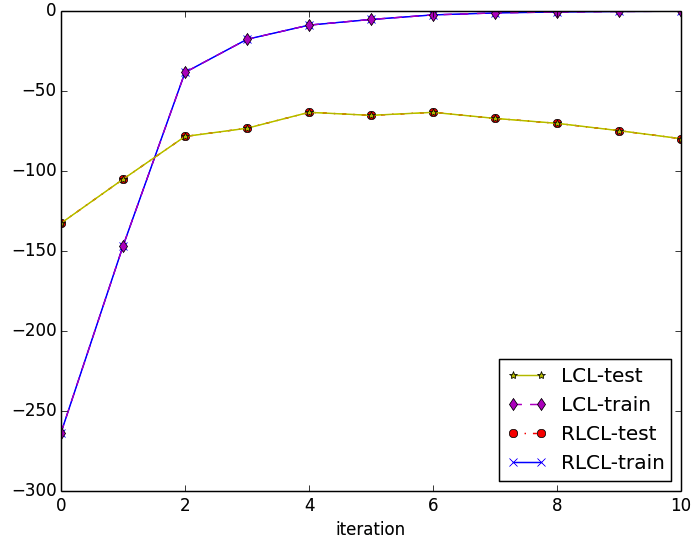
\includegraphics[width=0.8\textwidth]{noreg.png}
\caption{LCL for train and test sets for the case of learning with no regularization, i.e. $\mu=0$.}
\end{figure}
In the second experiment, we omitted the search for initial value for the parameter vector $\beta$ and instead, used a constant value of 0.1. For the regularization parameter $\mu$, we performed grid search over the set of values $[.001,.01,.1,1,10,100,1000]$ with 3-fold cross validation over the train set. Figure {\ref{figNoBeta0}} plots the LCL and RLCL for both train and test sets.

\begin{figure}[h!]
\label{figNoBeta0}
\centering
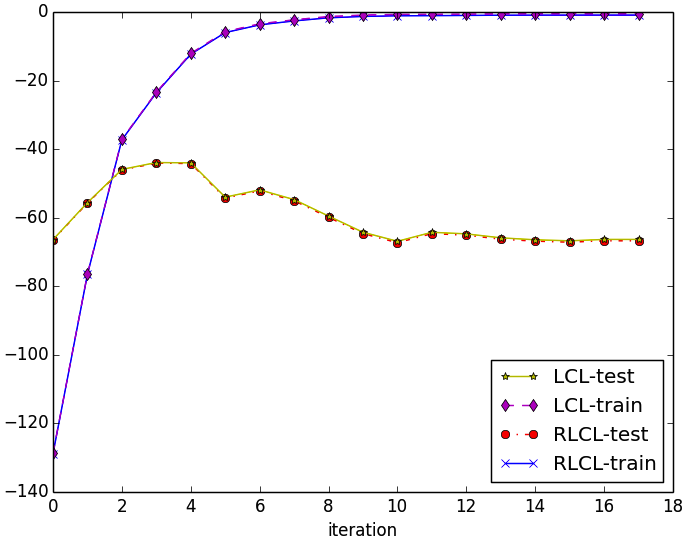
\includegraphics[width=0.8\textwidth]{nobeta0.png}
\caption{LCL and RLCL for train and test sets for the case with no search over initial weight values.}
\end{figure}



\section{Findings and Lessons Learned}
\subsection{Numerical Issues and Preprocessing}
\subsection{Overfitting}
\subsection{Model Selection}
\subsection{Trade-off Between Mini-Batch size and Rate of Convergence}

\end{document}

